\documentclass{beamer}

% Theme choice
\usetheme{Madrid}

% Optional packages
\usepackage{graphicx} % For including images
\usepackage{amsmath}  % For math symbols and formulas
\usepackage{hyperref} % For hyperlinks
\usepackage{listings}
\usepackage{xcolor}
\usepackage[T1]{fontenc}

\lstdefinestyle{CStyle}{
  language=C,                    % Set the language to C
  basicstyle=\ttfamily\footnotesize\linespread{0.9}\tiny, % Set font style and size
  keywordstyle=\color{blue},      % Color of keywords
  commentstyle=\color{gray},      % Color of comments
  stringstyle=\color{red},        % Color of strings
  showstringspaces=false,         % Do not mark spaces in strings
  breaklines=true,                % Enable line breaks at appropriate places
  breakatwhitespace=false,        % Break lines at any character, not just whitespace
  numbers=left,                   % Show line numbers on the left
  numberstyle=\tiny\color{gray},  % Style for line numbers
  tabsize=4,                      % Set tab width
  keepspaces=true,                % Keep indentation spaces
  frame=single,                   % Add a border around the code
  aboveskip=0pt,                  % Reduce space above the code block
  belowskip=0pt,                   % Reduce space below the code block
  xleftmargin=7.5pt,                      % Add left padding (approx. 2.8mm or 10px)
  xrightmargin=15pt,                      % Add left padding (approx. 2.8mm or 10px)
}

\AtBeginSection[]{
  \begin{frame}
    \centering
    \Huge\insertsection
  \end{frame}
}

% Title, author, date, and institute (optional)
\title[Parallel Programming. MPI (detailed API overview)]{Parallel Programming course. MPI (detailed API overview)}
\author{Obolenskiy Arseniy, Nesterov Alexander}
\institute{Nizhny Novgorod State University}

\date{\today} % or \date{Month Day, Year}

% Redefine the footline to display both the short title and the university name
\setbeamertemplate{footline}{
  \leavevmode%
  \hbox{%
    \begin{beamercolorbox}[wd=.45\paperwidth,ht=2.5ex,dp=1ex,leftskip=1em,center]{author in head/foot}%
        \usebeamerfont{author in head/foot}\insertshortinstitute % Displays the university name
    \end{beamercolorbox}%
    \begin{beamercolorbox}[wd=.45\paperwidth,ht=2.5ex,dp=1ex,leftskip=1em,center]{author in head/foot}%
      \usebeamerfont{author in head/foot}\insertshorttitle % Displays the short title
    \end{beamercolorbox}%
    \begin{beamercolorbox}[wd=.1\paperwidth,ht=2.5ex,dp=1ex,rightskip=1em,center]{author in head/foot}%
      \usebeamerfont{author in head/foot}\insertframenumber{} / \inserttotalframenumber
    \end{beamercolorbox}}%
  \vskip0pt%
}

\begin{document}

\begin{frame}
    \titlepage
\end{frame}

\begin{frame}{Contents}
    \tableofcontents
\end{frame}

\section{Advanced Send/Receive API}

\begin{frame}{Why Using \texttt{MPI\_Send} and \texttt{MPI\_Recv} Is Not Enough?}
  Blocking Operations \texttt{MPI\_Send} and \texttt{MPI\_Recv} are blocking, causing processes to wait until communication completes.
  So they are the reason of:
  \begin{itemize}
    \item \textbf{Performance Bottlenecks:} Blocking calls can lead to idle CPU time, reducing parallel efficiency.
    \item \textbf{Lack of Overlap:} Cannot overlap computation with communication, limiting optimization opportunities.
    \item \textbf{Scalability Issues:} As the number of processes increases, blocking operations can significantly degrade performance.
  \end{itemize}
\end{frame}

\begin{frame}{\texttt{MPI\_Isend}}
  Non-Blocking Send function. Initiates a send operation that returns immediately.

  {
    \footnotesize
    \texttt{int MPI\_Isend(const void *buf, int count, MPI\_Datatype datatype, int dest, int tag, MPI\_Comm comm, MPI\_Request *request);} \\
  }

  Parameters:

  \begin{itemize}
    \item buf: Initial address of send buffer
    \item count: Number of elements to send
    \item datatype: Data type of each send buffer element
    \item dest: Rank of destination process
    \item tag: Message tag
    \item comm: Communicator
    \item request: Communication request handle
  \end{itemize}
  {\footnotesize Usage: Allows the sender to proceed with computation while the message is being sent.}
\end{frame}

\begin{frame}{\texttt{MPI\_Irecv}}
  Non-Blocking Receive function. Initiates a receive operation that returns immediately.

  {
    \footnotesize
    \texttt{int MPI\_Irecv(void *buf, int count, MPI\_Datatype datatype, int source, int tag, MPI\_Comm comm, MPI\_Request *request);} \\
  }

  Parameters:

  \begin{itemize}
    \item buf: Initial address of receive buffer
    \item count: Maximum number of elements to receive
    \item datatype: Data type of each receive buffer element
    \item source: Rank of source process or \texttt{MPI\_ANY\_SOURCE}
    \item tag: Message tag or \texttt{MPI\_ANY\_TAG}
    \item comm: Communicator
    \item request: Communication request handle
  \end{itemize}
  {\footnotesize Usage: Allows the receiver to proceed with computation while waiting for the message.}
\end{frame}

\section{Synchronization}

\begin{frame}{What is synchronization in MPI?}
  Synchronization mechanisms are essential to coordinating processes.
  Sometimes we need to ensure that particular action has been already completed.

  Synchronization facts:

  \begin{itemize}
    \item Process Coordination: Mechanism to ensure processes reach a certain point before proceeding
    \item Data Consistency: Ensures all processes have consistent data before computations
    \item Types of Synchronization:
    \begin{itemize}
      \item Point-to-point synchronization: It involves explicit sending and receiving of messages between two processes using functions like \texttt{MPI\_Send} and \texttt{MPI\_Recv}
      \item Collective synchronization: Collective operations (see next slides) are used, where all processes must participate
    \end{itemize}
    \item Importance: Prevents race conditions and ensures program correctness
  \end{itemize}
\end{frame}

\begin{frame}{\texttt{MPI\_Barrier}}
  Global Synchronization function. It blocks processes until all of them have reached the barrier.

  {
    \footnotesize
    \texttt{int MPI\_Barrier(MPI\_Comm comm);} \\
  }

  Usage:

  \begin{itemize}
    \item Ensures all processes have completed preceding computations
    \item Commonly used before timing code segments for performance measurement
    \item Typical use case: Synchronize before starting a collective operation
  \end{itemize}
\end{frame}

\section{Collective operations}

\begin{frame}{Collective operations}
  Operations involving all processes within a communicator.

  Characteristics:
  \begin{itemize}
    \item Implicit synchronization among processes.
    \item Cannot be initiated between subsets unless a new communicator is created.
  \end{itemize}

  Examples:
  \begin{itemize}
    \item Data movement operations (e.g., \texttt{MPI\_Bcast}, \texttt{MPI\_Gather}).
    \item Reduction operations (e.g., \texttt{MPI\_Reduce}, \texttt{MPI\_Allreduce}).
  \end{itemize}

  Benefits (why use them instead of send/recv?):
  \begin{itemize}
    \item Optimized for underlying hardware and common user scenarios.
    \item Simplifies code and improves readability.
  \end{itemize}
\end{frame}

\begin{frame}{Broadcast (\texttt{MPI\_Bcast})}
  Send data from one process to all other processes.

  {
    \footnotesize
    \texttt{int MPI\_Bcast(void *buffer, int count, MPI\_Datatype datatype, int root, MPI\_Comm comm);} \\
  }

  \begin{minipage}[t]{0.6\textwidth}
    Parameters:
    \begin{itemize}
      \item buffer: Starting address of buffer.
      \item count: Number of entries in buffer.
      \item datatype: Data type of buffer elements.
      \item root: Rank of broadcast root.
      \item comm: Communicator.
    \end{itemize}
  \end{minipage}
  \hfill
  \begin{minipage}[t]{0.35\textwidth}
    \begin{figure}[h]
      \includegraphics[]{images/broadcast.png}
    \end{figure}
  \end{minipage}
  {\footnotesize Source: \href{https://pdc-support.github.io/introduction-to-mpi/07-collective/index.html}{https://pdc-support.github.io/introduction-to-mpi/07-collective/index.html}}
\end{frame}

\begin{frame}{Reduction (\texttt{MPI\_Reduce})}
  Perform a global reduction operation (e.g., sum, max) across all processes. Calculate the total sum of values distributed across processes.

  Can be seen as the opposite operation to broadcast.

  {
    \footnotesize
    \texttt{int MPI\_Reduce(const void *sendbuf, void *recvbuf, int count, MPI\_Datatype datatype, MPI\_Op op, int root, MPI\_Comm comm);} \\
  }

  \begin{minipage}[t]{0.2\textwidth}
    Supported operations:
    \begin{itemize}
      \item \texttt{MPI\_SUM}
      \item \texttt{MPI\_PROD}
      \item \texttt{MPI\_MAX}
      \item \texttt{MPI\_MIN}
    \end{itemize}
  \end{minipage}
  \hfill
  \begin{minipage}[t]{0.75\textwidth}
    \begin{figure}[h]
      \includegraphics[]{images/reduction.png}
    \end{figure}
  \end{minipage}
  {\footnotesize Source: \href{https://pdc-support.github.io/introduction-to-mpi/07-collective/index.html}{https://pdc-support.github.io/introduction-to-mpi/07-collective/index.html}}
\end{frame}

\begin{frame}{\texttt{MPI\_Gather}}
  Collect data from all processes to a single root process.

  {
    \footnotesize
    \texttt{int MPI\_Gather(const void *sendbuf, int sendcount, MPI\_Datatype sendtype, void *recvbuf, int recvcount, MPI\_Datatype recvtype, int root, MPI\_Comm comm);} \\
  }

  \begin{minipage}[t]{0.6\textwidth}
    Parameters:
    \begin{itemize}
      \item sendbuf: Starting address of send buffer.
      \item recvbuf: Starting address of receive buffer (significant only at root).
    \end{itemize}
  \end{minipage}
  \hfill
  \begin{minipage}[t]{0.35\textwidth}
    \begin{figure}[h]
      \includegraphics[]{images/gather.png}
    \end{figure}
  \end{minipage}
  {\footnotesize Source: \href{https://pdc-support.github.io/introduction-to-mpi/07-collective/index.html}{https://pdc-support.github.io/introduction-to-mpi/07-collective/index.html}}
\end{frame}

\begin{frame}{\texttt{MPI\_Scatter}}
  Distribute distinct chunks of data from root to all processes.

  {
    \footnotesize
    \texttt{int MPI\_Scatter(const void *sendbuf, int sendcount, MPI\_Datatype sendtype, void *recvbuf, int recvcount, MPI\_Datatype recvtype, int root, MPI\_Comm comm);} \\
  }

  \begin{minipage}[t]{0.6\textwidth}
    Parameters:
    \begin{itemize}
      \item \texttt{sendbuf}: Starting address of send buffer (significant only at root).
      \item \texttt{recvbuf}: Starting address of receive buffer.
    \end{itemize}
  \end{minipage}
  \hfill
  \begin{minipage}[t]{0.35\textwidth}
    \begin{figure}[h]
      \includegraphics[]{images/scatter.png}
    \end{figure}
  \end{minipage}
  {\footnotesize Source: \href{https://pdc-support.github.io/introduction-to-mpi/07-collective/index.html}{https://pdc-support.github.io/introduction-to-mpi/07-collective/index.html}}
\end{frame}

\begin{frame}{\texttt{MPI\_AllGather}}
  Gather data from all processes and distributes the combined data to all processes.

  {
    \footnotesize
    \texttt{int MPI\_Allgather(const void *sendbuf, int sendcount, MPI\_Datatype sendtype, void *recvbuf, int recvcount, MPI\_Datatype recvtype, MPI\_Comm comm);} \\
  }

  \begin{minipage}[t]{0.6\textwidth}
    Parameters:
    \begin{itemize}
      \item sendbuf: Starting address of send buffer
      \item sendcount / sendtype: Number and type of elements contributed by each process
      \item recvbuf: Starting address of receive buffer
      \item recvcount / recvtype: Number and type of elements received from each process
    \end{itemize}
  \end{minipage}
  \hfill
  \begin{minipage}[t]{0.35\textwidth}
    \begin{figure}[h]
      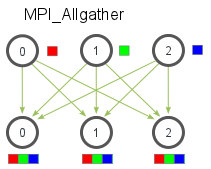
\includegraphics[scale=0.6]{images/allgather.png}
    \end{figure}
  \end{minipage}

  {\footnotesize Source: \href{https://mpitutorial.com/tutorials/mpi-scatter-gather-and-allgather/}{https://mpitutorial.com/tutorials/mpi-scatter-gather-and-allgather/}}
\end{frame}

\begin{frame}{All-to-All (\texttt{MPI\_Alltoall})}
  Description: Each process sends data to and receives data from all other processes. It can be seen as transposing a matrix distributed across processes.

  {
    \footnotesize
    \texttt{int MPI\_Alltoall(const void *sendbuf, int sendcount, MPI\_Datatype sendtype, void *recvbuf, int recvcount, MPI\_Datatype recvtype, MPI\_Comm comm);} \\
  }

  Note: This operation is communication-intensive.
\end{frame}

\begin{frame}{All API have not blocking versions}
  Non-Blocking collectives operations allow overlapping communication with computation.

  Examples:
  \begin{itemize}
    \item \texttt{MPI\_Ibcast}: Non-blocking broadcast.
    \item \texttt{MPI\_Ireduce}: Non-blocking reduction.
    \item \texttt{MPI\_Iallgather}: Non-blocking all-gather.
  \end{itemize}

  \texttt{int MPI\_Ibcast(void *buffer, int count, MPI\_Datatype datatype, int root, MPI\_Comm comm, MPI\_Request *request);}

  \texttt{int MPI\_Ireduce(const void *sendbuf, void *recvbuf, int count, MPI\_Datatype datatype, MPI\_Op op, int root, MPI\_Comm comm, MPI\_Request *request);}

  Usage flow is the same as for \texttt{MPI\_Isend}/\texttt{MPI\_Irecv}: Initiate the operation and later wait for its completion using \texttt{MPI\_Wait} or \texttt{MPI\_Test}.
\end{frame}

\begin{frame}
    \centering
    \Huge{Thank You!}
\end{frame}

\begin{frame}{References}
  \begin{enumerate}
    \item MPI Standard \href{https://www.mpi-forum.org/docs/}{https://www.mpi-forum.org/docs/}
    \item Open MPI v4.0.7 documentation: \href{https://www.open-mpi.org/doc/v4.0/}{https://www.open-mpi.org/doc/v4.0/}
    \item MPI Scatter, Gather, and Allgather: \href{https://mpitutorial.com/tutorials/mpi-scatter-gather-and-allgather/}{https://mpitutorial.com/tutorials/mpi-scatter-gather-and-allgather/}
  \end{enumerate}
\end{frame}

\end{document}
